\documentclass[a4paper,12pt,titlepage]{article}

\usepackage[utf8]{inputenc}
\usepackage[spanish]{babel}
\usepackage{graphics}

\begin{document}
\begin{center}

\begin{huge}
	\textbf{Trabajo Práctico Especial} 
\end{huge}

\vspace{20pt}

\begin{Huge}
	Programación Orientada a Objetos
\end{Huge}

\vspace{12pt}

\begin{large}
	Grupo 7
\end{large}

\end{center}

\section{Diseño}

\subsection{Estructura Básica}

Se modeló el juego Sokoban bajo el paradigma orientado a objetos.

Lo primero que definimos fué una clase \textbf{Game} que represente partidas de Sokoban. Un objeto de esta clase tiene atributos tales como nombre del usuario que está jugando, nombre del nivel, e información que nos permita decidir si el jugador ha ganado o no.

En un juego tenemos elementos (los cuales todos heredan de una clase \textbf{GameElement}), que los dividimos entre dos tipos: \textbf{GameTile}, una baldoza del juego (esto incluye los agujeros, paredes, y objetivos), y \textbf{GameObject}, que son los objetos que pueden estar arriba de una baldoza (el personaje del jugador y las cajas).

Dentro de un objeto \textbf{Game} debe existir un conjunto de \textbf{GameTile}s, almacenados en una matriz en nuestra implementación, representando las baldozas de un nivel de Sokoban. Debido a que un \textbf{GameObject} sólo puede estar arriba de una \textbf{GameTile}, almacenamos en cada \textbf{GameTile} información sobre quién es el \textbf{GameObject} que está encima de ella.

\newpage
\subsection{Diagrama UML}

\begin{center}
	\begin{figure}[h]
		\center 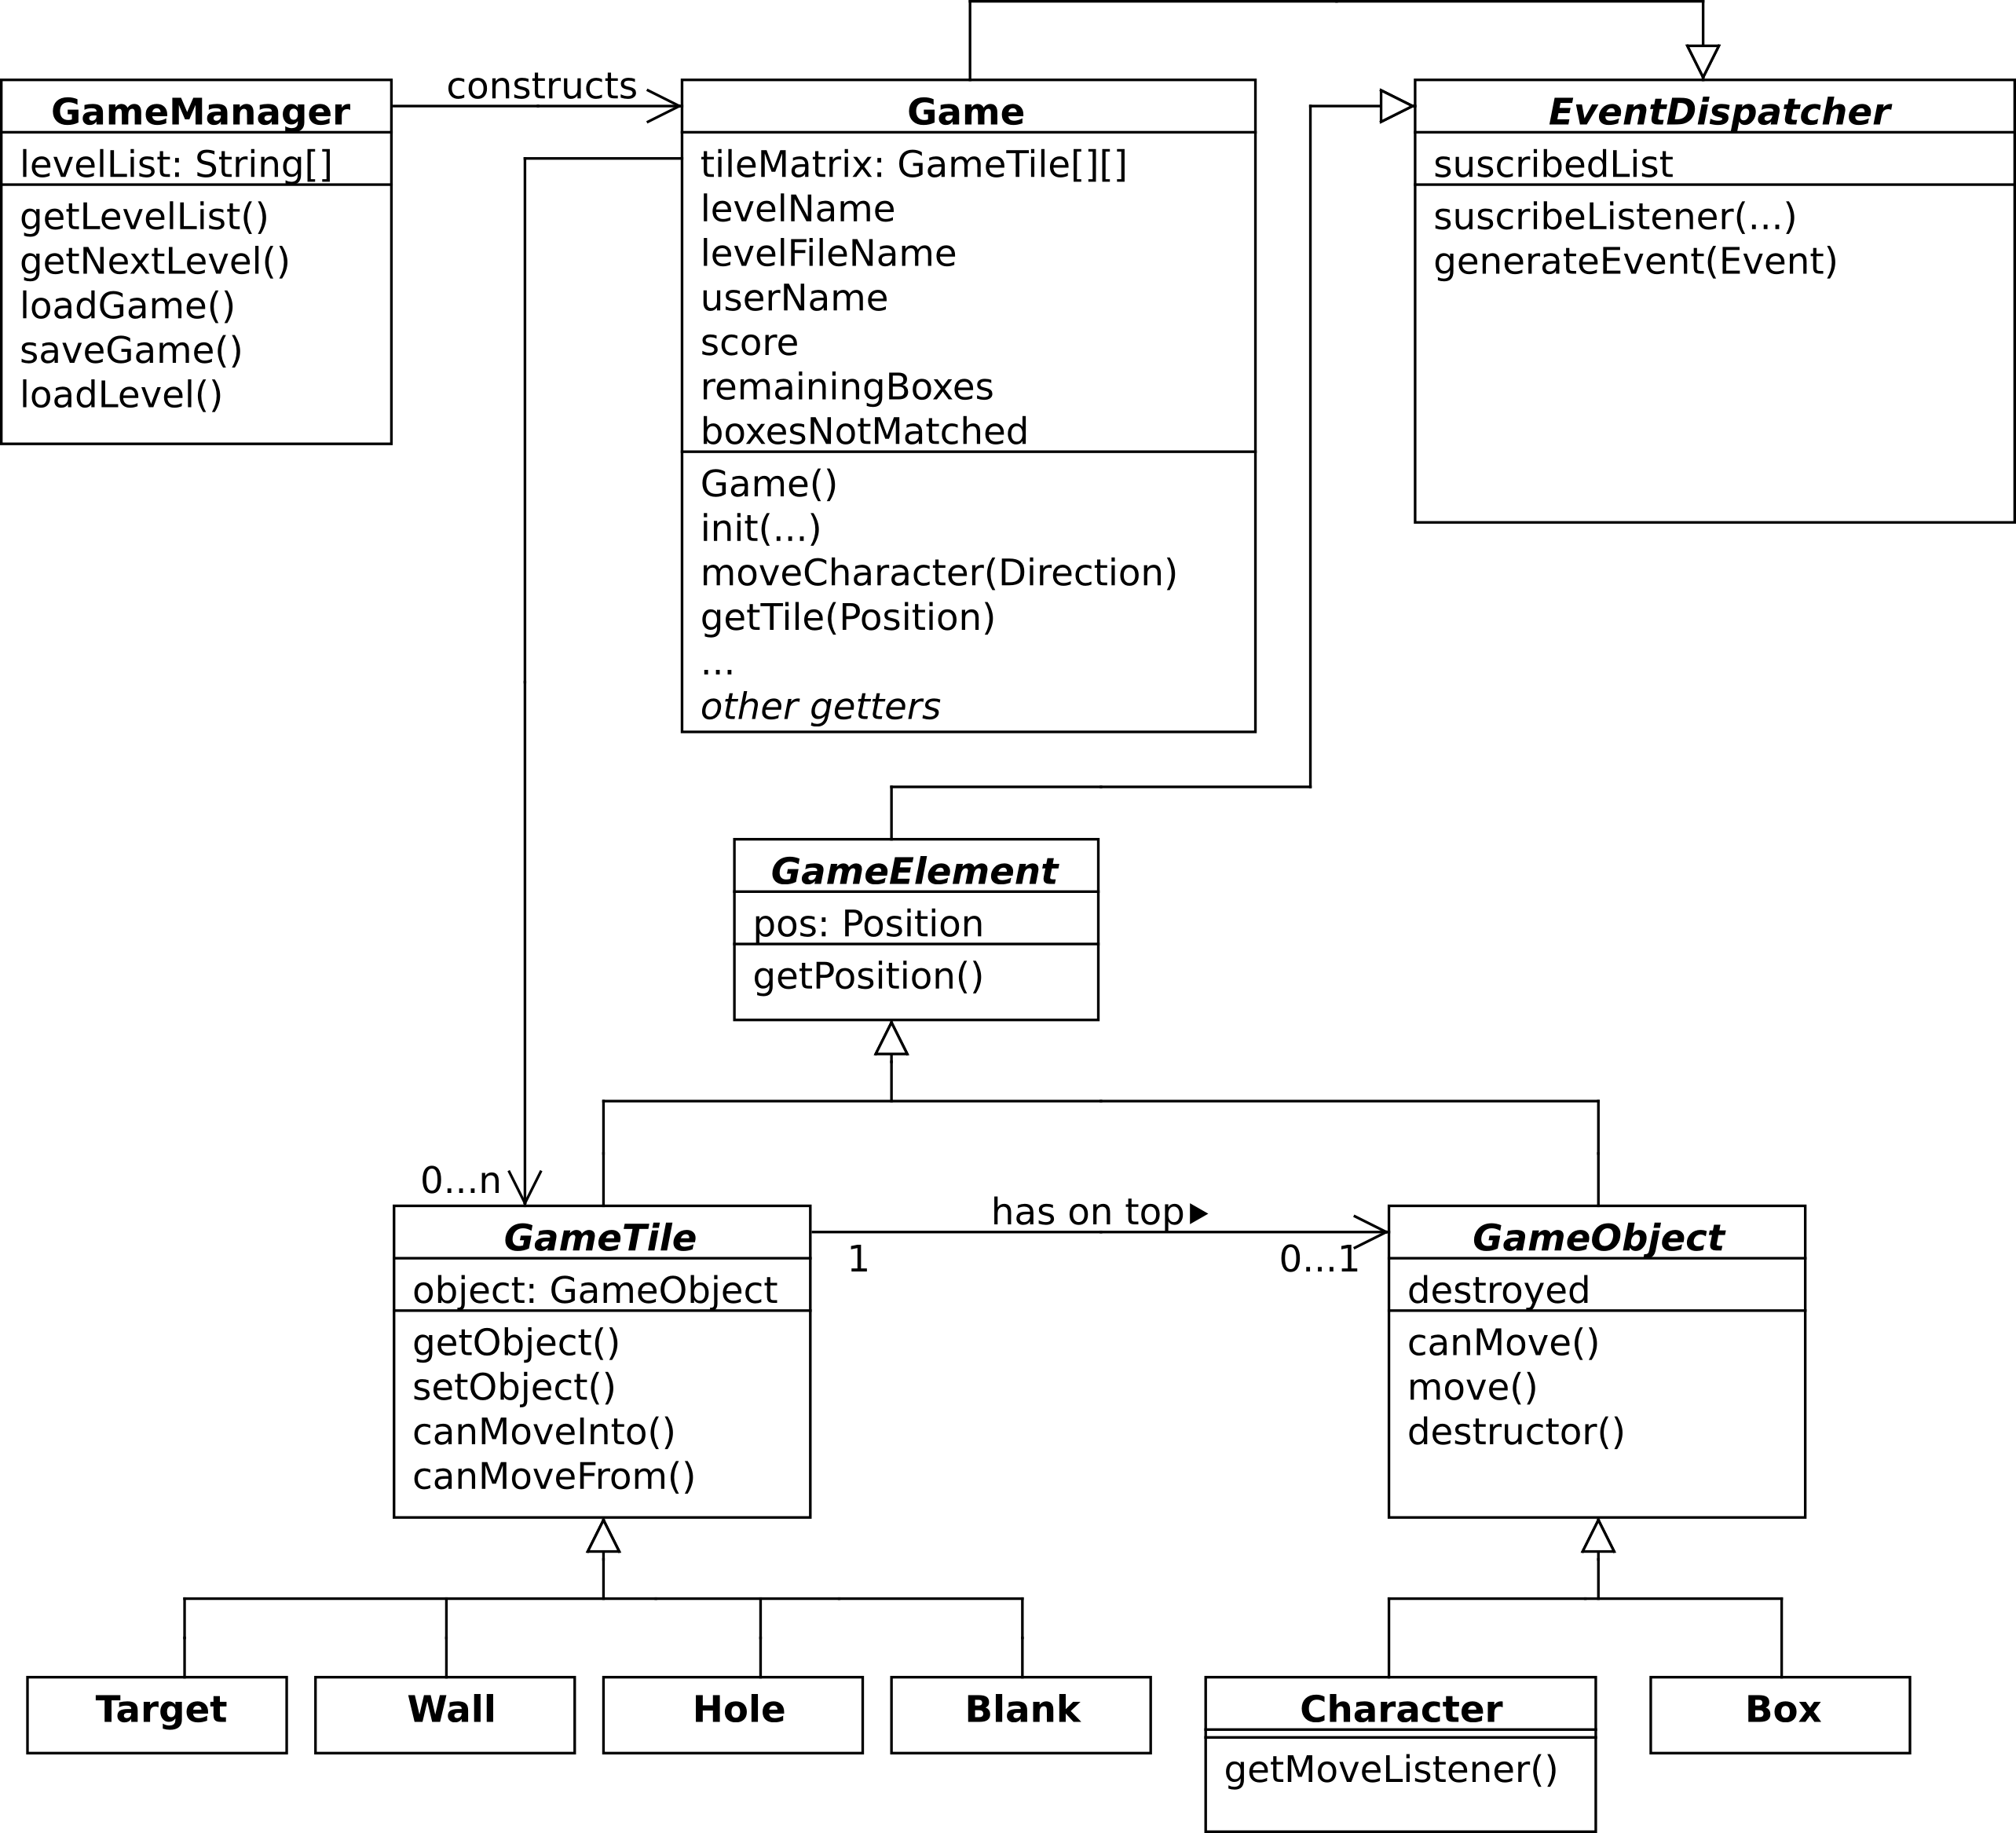
\includegraphics{ClassDiagram.png}
		\caption{Diagrama de clases}
	\end{figure}
\end{center}

\subsection{Eventos}

La comunicación interna entre objetos de \textbf{gamelogic} varía entre pasaje de mensajes y lanzamiento de \textbf{Event}s. Este modelo es una implementación del patrón \textbf{\emph{Observer}} en la que objetos que implementan la interfaz \textbf{EventListener} se suscriben a un \textbf{EventDispatcher}, encargado de notificar cada vez que un \textbf{Event} es lanzado.

La comunicación al exterior acerca de cambios de estado del juego se realiza puramente a través de este tipo de eventos. Movimiento de objetos, notificaciones de que el juego terminó, cambio del puntaje, son ejemplos de las notificaciones que nuestro \emph{backend} emite. Es responsabilidad del frontend responder a estos eventos. Por otro lado, el \emph{backend} no escucha a eventos externos, sólo responde a pasaje de mensajes. Sí escucha a eventos internos, lo que se describirá posteriormente.

\subsection{Movimiento de \textbf{GameObject}s}

Al recibir un evento del tipo \textbf{MoveCharacterEvent}, que representa una orden de moverse en determinada dirección, el \textbf{Character} instanciado en este juego pedirá información suficiente para saber si es posible realizar un movimiento.
Este evento contiene una referencia a \textbf{Game} y dispara el método \emph{canMove()} del \textbf{Character} y los pasos que éste realiza para responder bien son:

\begin{itemize}
 \item Preguntar si el \textbf{GameTile} vecino tiene un objeto arriba
 \begin{itemize}
  \item Si contiene un objeto, determinar si se puede mover en esa misma dirección llamando al método \textit{canMove()} del \textbf{GameObject}.
 \end{itemize}
 \item Preguntar al \textbf{GameTile} debajo suyo si puede salir en esa dirección.
 \item Preguntar al \textbf{GameTile} vecino si se puede mover entrando en esa dirección.
\end{itemize}

Estas comprobaciones son realizadas por pasaje de mensajes y no de eventos, debido a que todas necesitan devolver un valor y por simplicidad no agregamos funciones de \emph{callback}.

Se utiliza un evento \textbf{moveCharacterEvent} interno para realizar esto para evitar que la instancia de \textbf{Game} mantenga información adicional acerca del \textbf{Character}. De este modo, \textbf{Game} sólo tiene una matriz de \textbf{GameTile}s. Esto fué decidido para evitar referencias desde el Game hacia el \textbf{Character}, para no dar saltos dentro del árbol de clases.

\subsection{Lógica del Estado del Juego}

Cada vez que el estado de un \textbf{GameElement} cambia, es disparado un evento de tipo \textbf{StateUpdatedEvent} informando que un \textbf{GameTile} dejó o pasó a tener un nuevo \textbf{GameObject} sobre él, o bien un \textbf{GameObject} actualizó su posición.

Los \textbf{GameTile}s de tipo \textbf{Target} además, disparan un evento \textbf{TargetMatchedEvent} cuando es posicionada una \textbf{Box} del mismo color sobre el tile, y un evento \textbf{TargetUnmatchedEvent} cuando una \textbf{Box} de su color deja la casilla. La clase \textbf{Game} escucha este tipo de eventos y al ser disparado uno, actualiza el contador del juego y en caso de que dispara un nuevo evento \textbf{ScoreUpdatedEvent}, avisando de un cambio en el puntaje del jugador. El orden en que ocurren estos cambios es el siguiente:

\begin{itemize}
	\item El \textbf{GameTile} del origen ha cambiado su estado: dejó de ser anfitrión de un \textbf{GameObject}.
	\item El \textbf{GameTile} destino ha cambiado su estado: contiene un \textbf{GameObject}.
	\item \textbf{GameObject} ha cambiado su estado: cambió su posición.
\end{itemize}

Asimismo, un \textbf{Hole} al recibir un \textbf{GameObject}, le manda un mensaje para avisarle que ha sido destruído. Un objeto al ser destruído manda un evento \textbf{DestroyedEvent}. Este tipo de eventos es escuchado internamente, debido a que \textbf{Game} debe disminuír un contador de \textbf{Box}es en el nivel y enviar eventos de tipo \textbf{GameOverEvent} si el objeto que cayó es el \textbf{Character}.

En caso de que se cumpla la condición de que la \emph{cantidad de cajas actuales en el nivel} sea igual a la \emph{cantidad de objetivos en el nivel con una caja de su color arriba} (ambas son atributos guardados en la instancia de \textbf{Game}), el juego fué ganado, y se lanza un event de tipo \textbf{GameFinishedEvent}

\subsection{Nuevas Partidas}

La creación de nuevos juegos se realiza usando el patrón de diseño \textbf{\emph{Factory}}. Una clase \textbf{GameManager} es encargada de leer datos sobre cómo crear un nuevo juego a partir de un archivo e instanciar un nuevo \textbf{Game} a partir de esos datos, ya sean estos de una partida guardada o no. La clase asegura que se instanciaran todos los \textbf{GameElement} que se lean del archivo (si el archivo no está corrupto, en cuyo caso se debe tirar una \textbf{Exception}), en orden especifico: primero los \textbf{GameTile}s y luego los \textbf{GameObject}s.

Esta clase permite ser extendida y sus métodos fueron subdivididos para que puedan ser sobreescritos o sobrecargados diferenciando las subclases de \textbf{GameElement} que son instanciadas. 

\subsection{Elementos Auxiliares del Juego}

Distintas clases del \emph{backend} sirven a la lógica del juego:

\begin{itemize}
    \item \textbf{Position}: objeto inmutable que representa una posición del tablero.
    \item \textbf{Direction}: objeto inmutable que representa una dirección en la que un \textbf{GameObject} puede moverse.
    \item \textbf{Color}: representación de un color por sus componentes RGB.
    \item \textbf{ElementType}: un enumerador para corresponder cada tipo de \textbf{GameObject} con un entero.
	\item \textbf{Highscores}: clase encargada de guardar los mejores puntajes dado el nombre del archivo del nivel.
\end{itemize}

\section{Desafíos Encontrados}

\subsection{Modelado Inicial}

Nos llevó varias horas ponernos de acuerdo en cómo representar los elementos del juego en una manera que se pudiera distinguir bien el \emph{backend} del \emph{frontend}. En un diseño original que estaba claramente fallado, el \emph{frontend} era una herramienta fundamental que necesitaba el \emph{backend} para generar nuevos juegos. Con esto no había independencia entre el backend y el frontend.

Heredamos de este modelado inicial el patrón \emph{\textbf{Factory}}, pero con una mejor independencia: la clase \textbf{GameManager} que construye \textbf{Game} y el resto de los \textbf{GameElements} fué dividida de manera tal que cualquier etapa de la formación del juego pueda ser sobreescrita y/o extendida por una clase hija.

\subsection{Diseño del Frontend}

Al adoptar el modelo MVC, nuestros modelos de \emph{backend} debían tener clases "hermanas" que las compusieran. En un principio, estuvimos tentados por la opción "imperativa", hacer un mapeo de los \emph{Strings} con los nombres de las clases del \emph{backend} hacia imágenes, con casteos para obtener más datos, como el color de las cajas. Abandonamos esta idea por parecernos una mala práctica y nos mantuvimos dentro del paradigma orientado a objetos.

La correcta separación entre la \emph{Vista} y el \emph{Controlador} requirió también de un refactoreo entero de ambos, debido a que nos aceleramos a intentar "tener algo andando".

\subsection{Implementación}

A medida que debíamos pasar del diseño a la programación, nos encontrabamos cada día con nuevos obstáculos: debates sobre si hacemos esto de tal o cual manera fueron muy abundantes durante el proceso y encontramos que varias decisiones requirieron que volviéramos a replantear nuestro diseño en un par de ocaciones.

En momentos, cuando encontramos un \emph{bug} importante durante la implementación, escribimos un \emph{Unit Test} para mostrar cómo debía ser la funcionalidad y corregir el código para que estas pruebas no fallaran. Esto probó ser muy eficiente y necesitar escribir el \emph{test} nos ayudaba a entender aún más claramente el funcionamiento del flujo de nuestro diseño.

\subsection{Trabajo en Equipo}

Luego del diseño inicial, fué cuestión de dividir bien el trabajo y en horas gran parte del juego estaba andando correctamente. 

\end{document}